%=======================================================================
%  Air Connectivity and Goods Trade: A Global IV Study, 1996-2023
%  Target: Transportation Research Part A: Policy and Practice (Elsevier)
%  Compile: pdflatex -> bibtex -> pdflatex x2   (bib: GACI_TRA_refs.bib)
%  Figures needed in project root:
%     GACI_base_map.png  GACI_implied_map.png
%     GACI_continent_trend.png  GACI_shock_map.png
%=======================================================================
\documentclass[review,3p,times]{elsarticle}

\usepackage{lineno,hyperref}
\usepackage{amsmath,amssymb}
\usepackage{graphicx}
\usepackage{booktabs}
\usepackage{threeparttable}
\usepackage{siunitx}
\usepackage{multirow}
\usepackage[flushleft]{threeparttablex}
\journal{Transportation Research Part A: Policy and Practice}

\newcommand{\sym}[1]{\rlap{$^{#1}$}}

\begin{document}

\begin{frontmatter}

\title{Global Air Connectivity and Trade Openness, 1996--2023}

\author[a]{Sunbin Yoo\corref{cor1}}
\ead{sunbinyoo.kyushu@gmail.com}
\cortext[cor1]{Corresponding author.}
\author[a]{[Co-author]}
\address[a]{[Affiliation], Kyushu University, Fukuoka, Japan}

\begin{abstract}
We estimate the causal effect of global air connectivity on merchandise
(goods) trade for a balanced panel of 184 countries over 1996--2023. Air
connectivity is measured by the Global Air Connectivity Index (GACI), a
network-centrality summary of each country's position in the world airport
network. Because airlines add routes where trade is already growing, we
isolate exogenous variation in connectivity using an instrument built from
each country's fixed natural-heritage endowment and the global tourism
cycle---leisure-driven air links that are unrelated to a country's
goods-trade fundamentals. Two-stage least squares with country and year fixed
effects yields a goods-trade-volume elasticity of $2.30$, which decomposes
exactly into a trade-intensity (openness) elasticity of $1.30$ and a GDP-scale
elasticity of $1.00$; the estimates are robust across alternative instruments
and falsification checks. Returns are highly uneven: the openness payoff to
connectivity declines with both baseline income and baseline connectivity, so
the marginal value of an additional air link is largest in poorer, remote, and
under-served economies---consistent with aviation substituting for weak
surface and maritime access---and smaller in already well-connected advanced
hubs. The same elasticity implies that abrupt connectivity collapses are
costly and that the relationship operates symmetrically in expansions and
contractions: the 2019--2020 COVID-19 shock, which cut connectivity in 140 of
177 countries, is associated with a goods-trade disruption on the order of
\$1.8 trillion (about 4.8\% of 2019 world goods trade), concentrated in major
gateway hubs. A partial-equilibrium counterfactual attributes about \$7.8
trillion of 2023 goods trade (roughly 17\% of the world total, or 7.4\% of
world GDP) to connectivity growth since 1996. The results identify airport and
route investment and air-service liberalisation as concrete, spillover-aware
levers for trade integration.
\end{abstract}

\begin{keyword}
Air connectivity \sep international trade \sep shift-share instrument \sep
network centrality \sep tourism \sep open skies
\end{keyword}

\end{frontmatter}

\linenumbers

%=======================================================================
\section{Introduction}
%=======================================================================
Air transport links move people far more than freight tonnage, yet a large
literature argues that passenger connectivity is itself an input to goods
trade: face-to-face contact lowers search and contracting costs
\citep{Cristea_2011,Belenkiy_2012,Startz_2016}, business travel diffuses
knowledge across borders \citep{Hovhannisyan_2015}, and dense air-link
networks raise local economic activity and integration
\citep{Brueckner_2003,Campante_2017}. The mechanism is information-economic:
trade in differentiated goods is organised through relationships and networks
\citep{Rauch_1999,Allen_2014}, and the costs of forming and maintaining those
relationships fall when two economies are easy to reach by air.

Estimating the \emph{causal} effect of air connectivity on trade is difficult
because connectivity is endogenous: airlines add routes where trade and income
are already growing. We address this with two design choices. First, we
measure connectivity not as a binary route opening but as a continuous,
network-based index---the Global Air Connectivity Index (GACI)---that captures
a country's centrality in the world airport network and therefore embeds
second-order (partner-of-partner) spillovers that bilateral
difference-in-differences designs miss. Second, we instrument connectivity with
a shift-share (Bartik) instrument \citep{GoldsmithPinkham_2020,Borusyak_2022}
that interacts a country's fixed \emph{natural and mixed} UNESCO World Heritage
endowment with the global time path of tourist demand. Heritage-driven leisure
demand shifts an airport's network position for reasons unrelated to the
country's goods-trade fundamentals, while the outcome---merchandise trade---
excludes services and tourism by construction, closing the most obvious
back-door from the instrument to the outcome.

Our headline estimate is a goods-trade-volume elasticity of $2.30$ with respect
to hub quality, which by the accounting identity
$\ln(\text{goods}) = \ln(\text{goods}/\text{GDP}) + \ln(\text{GDP})$ splits
exactly into a trade-\emph{intensity} elasticity of $1.30$ and a GDP-scale
elasticity of $1.00$. We report the intensity channel as the headline because
it is the pure openness effect, net of the income-scale channel. The estimate
is robust across a sequence of over-identification and falsification tests,
including a completely independent air/sea-distance instrument in the spirit of
\citet{Frankel_1999} and \citet{Feyrer_2019} that reproduces the same volume
elasticity. We then characterise heterogeneity and quantify the aggregate
contribution of two decades of connectivity growth.

The paper contributes to three literatures: the economics of air transport and
development \citep{Brueckner_2003,Campante_2017}; the trade-and-distance
identification literature \citep{Frankel_1999,Feyrer_2019}; and the methodology
of shift-share inference \citep{GoldsmithPinkham_2020,Adao_2019,Borusyak_2022}.
Relative to prior work it offers a globally scalable, continuous,
spillover-aware connectivity treatment with a transparent and testable
exclusion restriction.

%=======================================================================
\section{Data}
%=======================================================================
\paragraph{Connectivity (GACI).} GACI is constructed from global airline
schedule data (OAG) by building, for each year, the world airport network and
summarising each country's centrality (degree, closeness, betweenness, and
capacity weights aggregated to the country level). We use two treatments: the
capacity-weighted \emph{mean} connectivity of a country's airports
($\ln\text{GACI}_{cwm}$, ``hub quality''), our headline measure, and the
country \emph{sum} ($\ln\text{GACI}_{sum}$, total connectivity), used for the
abrupt one-year shock exercise where the mean is too volatile. Airport
coordinates are merged from OpenFlights and OurAirports; country boundaries for
the maps are from Natural Earth.

\paragraph{Outcome.} Goods (merchandise) trade as a share of GDP (World Bank
WDI, \texttt{TG.VAL.TOTL.GD.ZS}). Services and tourism receipts are excluded by
construction. We study three trade outcomes---log goods volume
($\ln\text{goods}$), log goods intensity/openness ($\ln(\text{goods}/\text{GDP})$),
and the goods-trade share in levels---plus log GDP per capita and log GDP.

\paragraph{Instrument inputs.} The fixed ``share'' is each country's cumulative
count of \emph{natural} and \emph{mixed} UNESCO World Heritage sites (UNESCO
World Heritage Centre). The global ``shift'' is world international tourist
arrivals (World Bank WDI \texttt{ST.INT.ARVL}, 1996--2019; extended to
2020--2023 with UNWTO figures), min--max scaled to $[0,1]$. The baseline
instrument is
\begin{equation}
\text{tourism\_int}_{it} \;=\; \underbrace{\widetilde{D}_t}_{\text{global tourism shift}}
\times \underbrace{\ln\!\bigl(1+H_i^{\text{nat+mix}}\bigr)}_{\text{fixed heritage share}},
\label{eq:instr}
\end{equation}
where $H_i^{\text{nat+mix}}$ is country $i$'s natural-plus-mixed heritage stock
and $\widetilde{D}_t$ is scaled world tourism demand. For robustness we also
build an independent air/sea-distance instrument (Section~\ref{sec:robust})
using the CERDI sea-distance database \citep{Bertoli_2016}.

\paragraph{Covariates and controls.} Population, GDP, and GDP per capita (WDI).
All specifications include country and year fixed effects; population enters as
a control. Summary statistics are in Appendix~\ref{app:sumstat}.

%=======================================================================
\section{Empirical strategy}
%=======================================================================
We estimate
\begin{equation}
y_{it} \;=\; \beta\,\ln\text{GACI}^{cwm}_{it} \;+\; \gamma\,\ln\text{pop}_{it}
\;+\; \alpha_i \;+\; \delta_t \;+\; \varepsilon_{it},
\label{eq:main}
\end{equation}
where $y_{it}$ is a trade or income outcome, $\alpha_i$ and $\delta_t$ are
country and year fixed effects, and $\ln\text{GACI}^{cwm}_{it}$ is instrumented
by Eq.~\eqref{eq:instr}. Identification comes from within-country variation in
hub quality driven by the interaction of a fixed heritage endowment with the
global tourism cycle, purged of country and year shocks.

The exclusion restriction requires that, conditional on fixed effects and
population, heritage-driven tourism demand affects goods trade \emph{only}
through air connectivity. Two features support it: (i) the outcome excludes the
services/tourism channel through which heritage could mechanically raise
exports; and (ii) natural and mixed heritage are geological/ecological
endowments, plausibly unrelated to a country's manufacturing or commodity
export base. We test exclusion directly in Section~\ref{sec:robust} by
over-identifying the model and by adding \emph{cultural} heritage, which is more
likely to co-move with development and should fail the test.

Standard errors are reported both heteroskedasticity-robust (in parentheses)
and clustered by country (in brackets). Because shift-share exposure varies
across countries, we also note the \citet{Adao_2019} concern that conventional
standard errors can understate uncertainty; our inferences are unchanged under
country clustering.

%=======================================================================
\section{Main results}
%=======================================================================
Table~\ref{tab:main} reports OLS and IV estimates of Eq.~\eqref{eq:main} for
the headline hub-quality treatment. The IV goods-volume elasticity is $2.30$
($p<0.01$); it decomposes exactly into a trade-intensity (openness) elasticity
of $1.30$ ($p<0.05$) and a GDP-scale elasticity of $1.00$, since
$\ln\text{goods} = \ln(\text{goods}/\text{GDP}) + \ln\text{GDP}$. IV exceeds
OLS, consistent with classical attenuation and with OLS mixing in
demand-driven route entry that is less trade-elastic than the leisure-driven
variation the instrument isolates. The first stage is strong
(Kleibergen--Paap $F=18.0$), addressing weak-instrument concerns. We treat the
intensity channel ($1.30$) as the headline causal object: it is the pure
openness effect of connectivity, net of income scale.

\begin{table}[t]
\centering
\caption{Main results: OLS vs.\ IV, hub-quality connectivity, 1996--2023.}
\label{tab:main}
\begin{threeparttable}
\small
\begin{tabular}{lccccc}
\toprule
 & \multicolumn{1}{c}{Goods} & \multicolumn{1}{c}{Goods} & \multicolumn{1}{c}{Goods}
 & \multicolumn{1}{c}{GDP} & \multicolumn{1}{c}{GDP} \\
 & \multicolumn{1}{c}{volume} & \multicolumn{1}{c}{intensity} & \multicolumn{1}{c}{share}
 & \multicolumn{1}{c}{per cap.} & \multicolumn{1}{c}{(level)} \\
 & \multicolumn{1}{c}{$\ln$} & \multicolumn{1}{c}{$\ln(g/Y)$} & \multicolumn{1}{c}{\%GDP}
 & \multicolumn{1}{c}{$\ln$} & \multicolumn{1}{c}{$\ln$} \\
\midrule
\multicolumn{6}{l}{\emph{Panel A. OLS}}\\
$\ln\text{GACI}_{cwm}$ & 1.144\sym{***} & 0.157\sym{***} & 14.71\sym{***} & 0.831\sym{***} & 0.987\sym{***} \\
\\
\multicolumn{6}{l}{\emph{Panel B. IV (2SLS)}}\\
$\ln\text{GACI}_{cwm}$ & 2.303\sym{***} & 1.302\sym{**} & 61.11 & 0.514 & 1.001 \\
\quad robust (s.e.)    & (0.776) & (0.662) & (46.43) & (0.475) & (0.680) \\
\quad cluster [s.e.]   & [1.762] & [1.269] & [83.01] & [1.000] & [1.467] \\
\midrule
First-stage KP $F$ & \multicolumn{5}{c}{18.0} \\
Country, Year FE   & Yes & Yes & Yes & Yes & Yes \\
Observations       & 4642 & 4642 & 4642 & 4642 & 4642 \\
\bottomrule
\end{tabular}
\begin{tablenotes}\footnotesize
\item Instrument: tourism\_int (Eq.~\ref{eq:instr}), global tourism demand
$\times$ fixed natural+mixed heritage. Robust s.e.\ in parentheses, country-
clustered s.e.\ in brackets. By the log identity, the volume elasticity
($2.303$) equals the intensity ($1.302$) plus GDP-scale ($1.001$) elasticities.
\sym{*}~$p<0.10$, \sym{**}~$p<0.05$, \sym{***}~$p<0.01$.
\end{tablenotes}
\end{threeparttable}
\end{table}

Figure~\ref{fig:basemap} maps the 2023 connectivity levels (high: United
States, China, the large European hubs); the implied intensity-channel trade
gain since 1996 is mapped in Figure~\ref{fig:impliedmap}.

\begin{figure}[t]
\centering
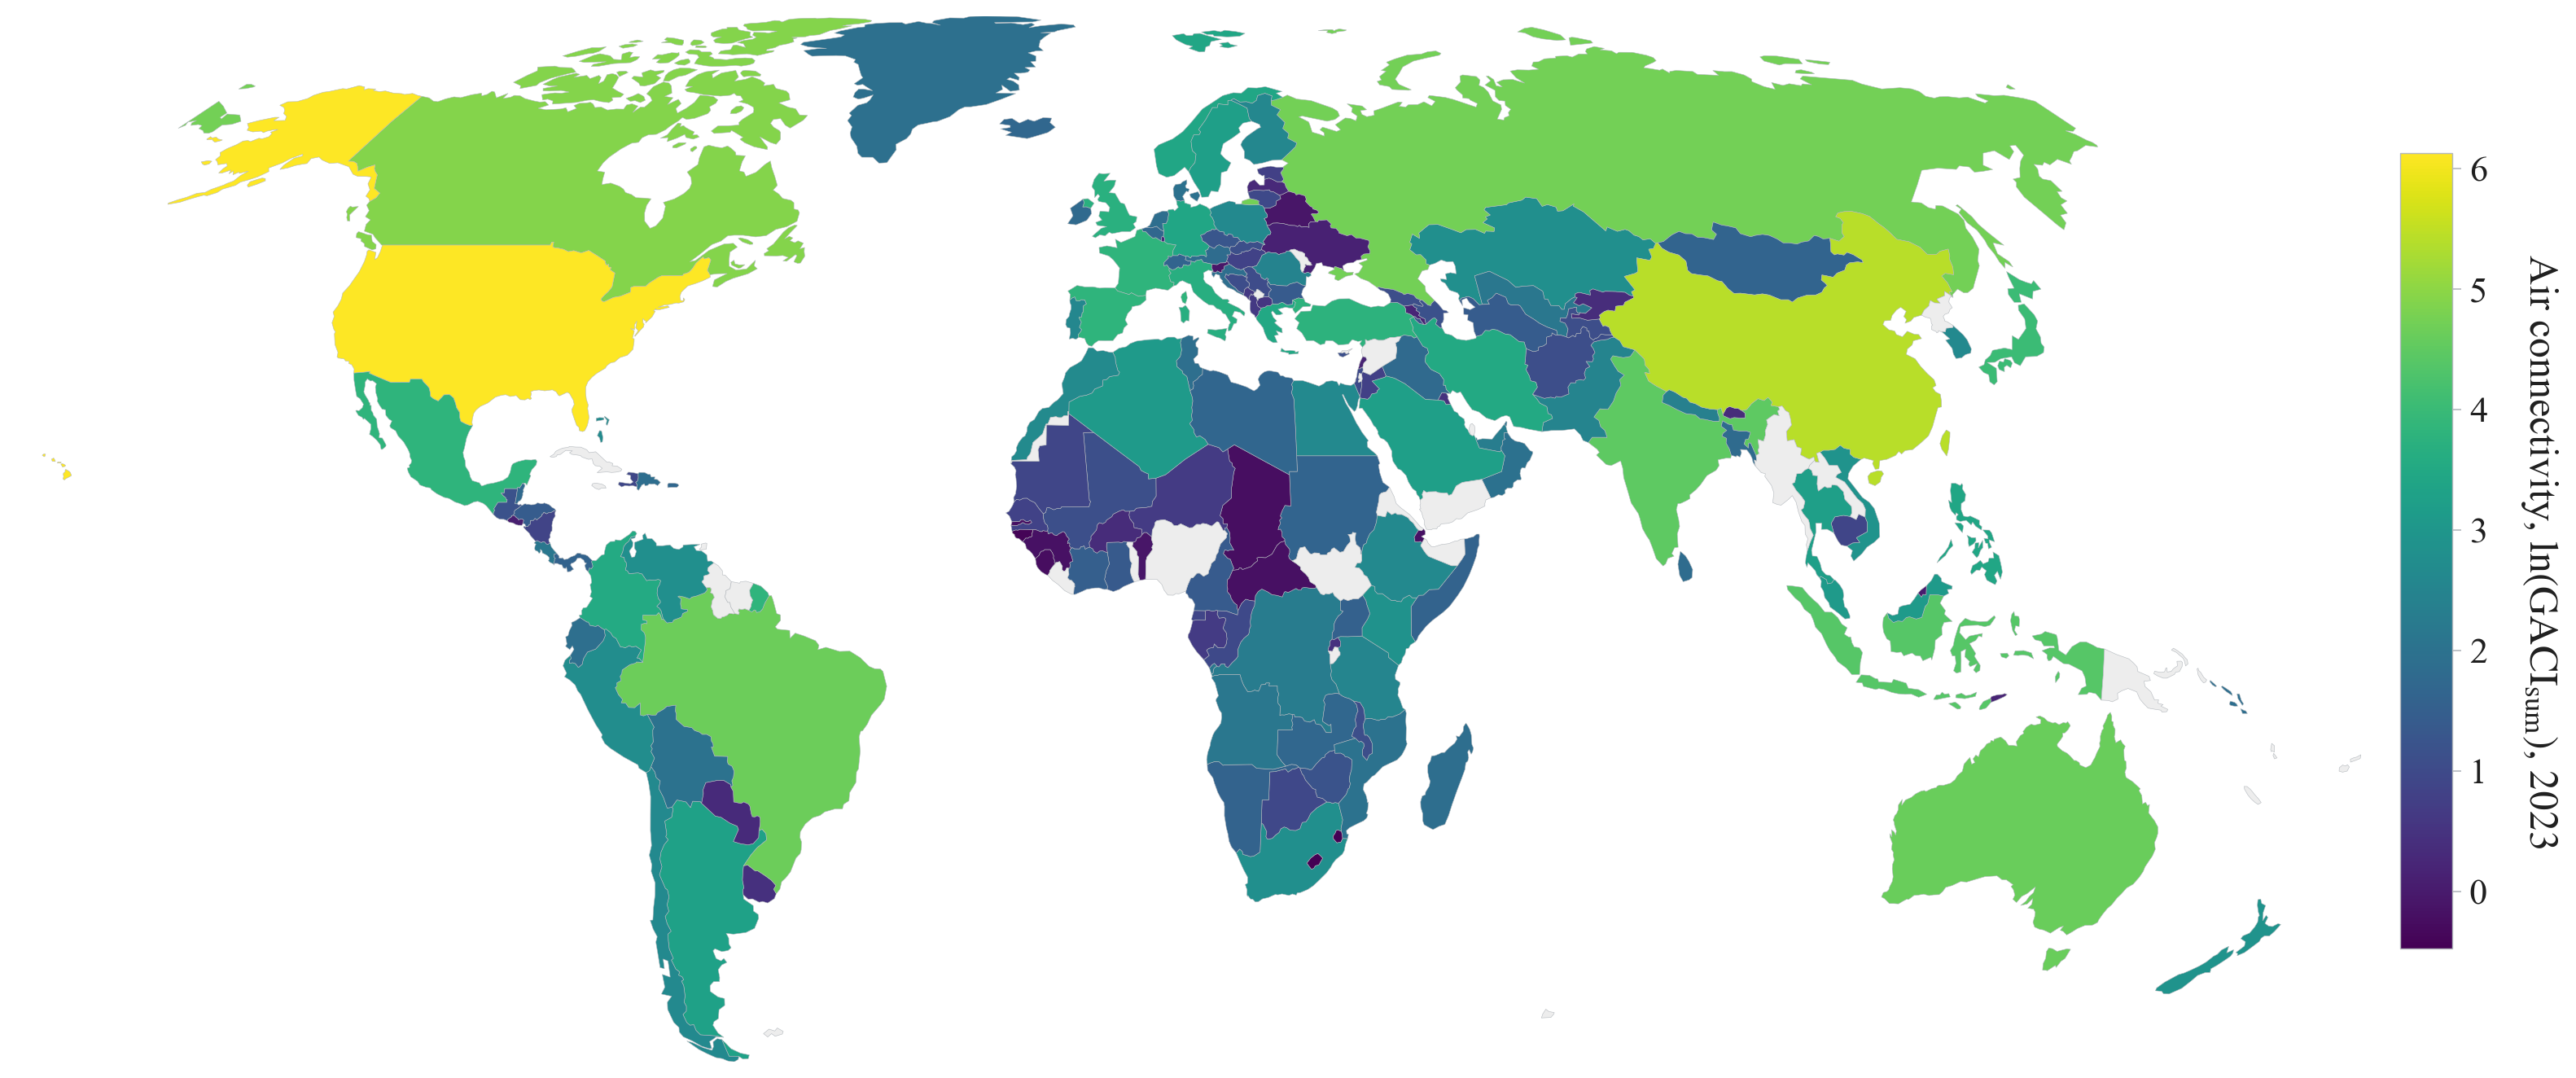
\includegraphics[width=0.92\linewidth]{GACI_base_map.png}
\caption{Air connectivity (GACI) levels, 2023. Yellow = highly connected
(United States, China, large European hubs).}
\label{fig:basemap}
\end{figure}

\begin{figure}[t]
\centering
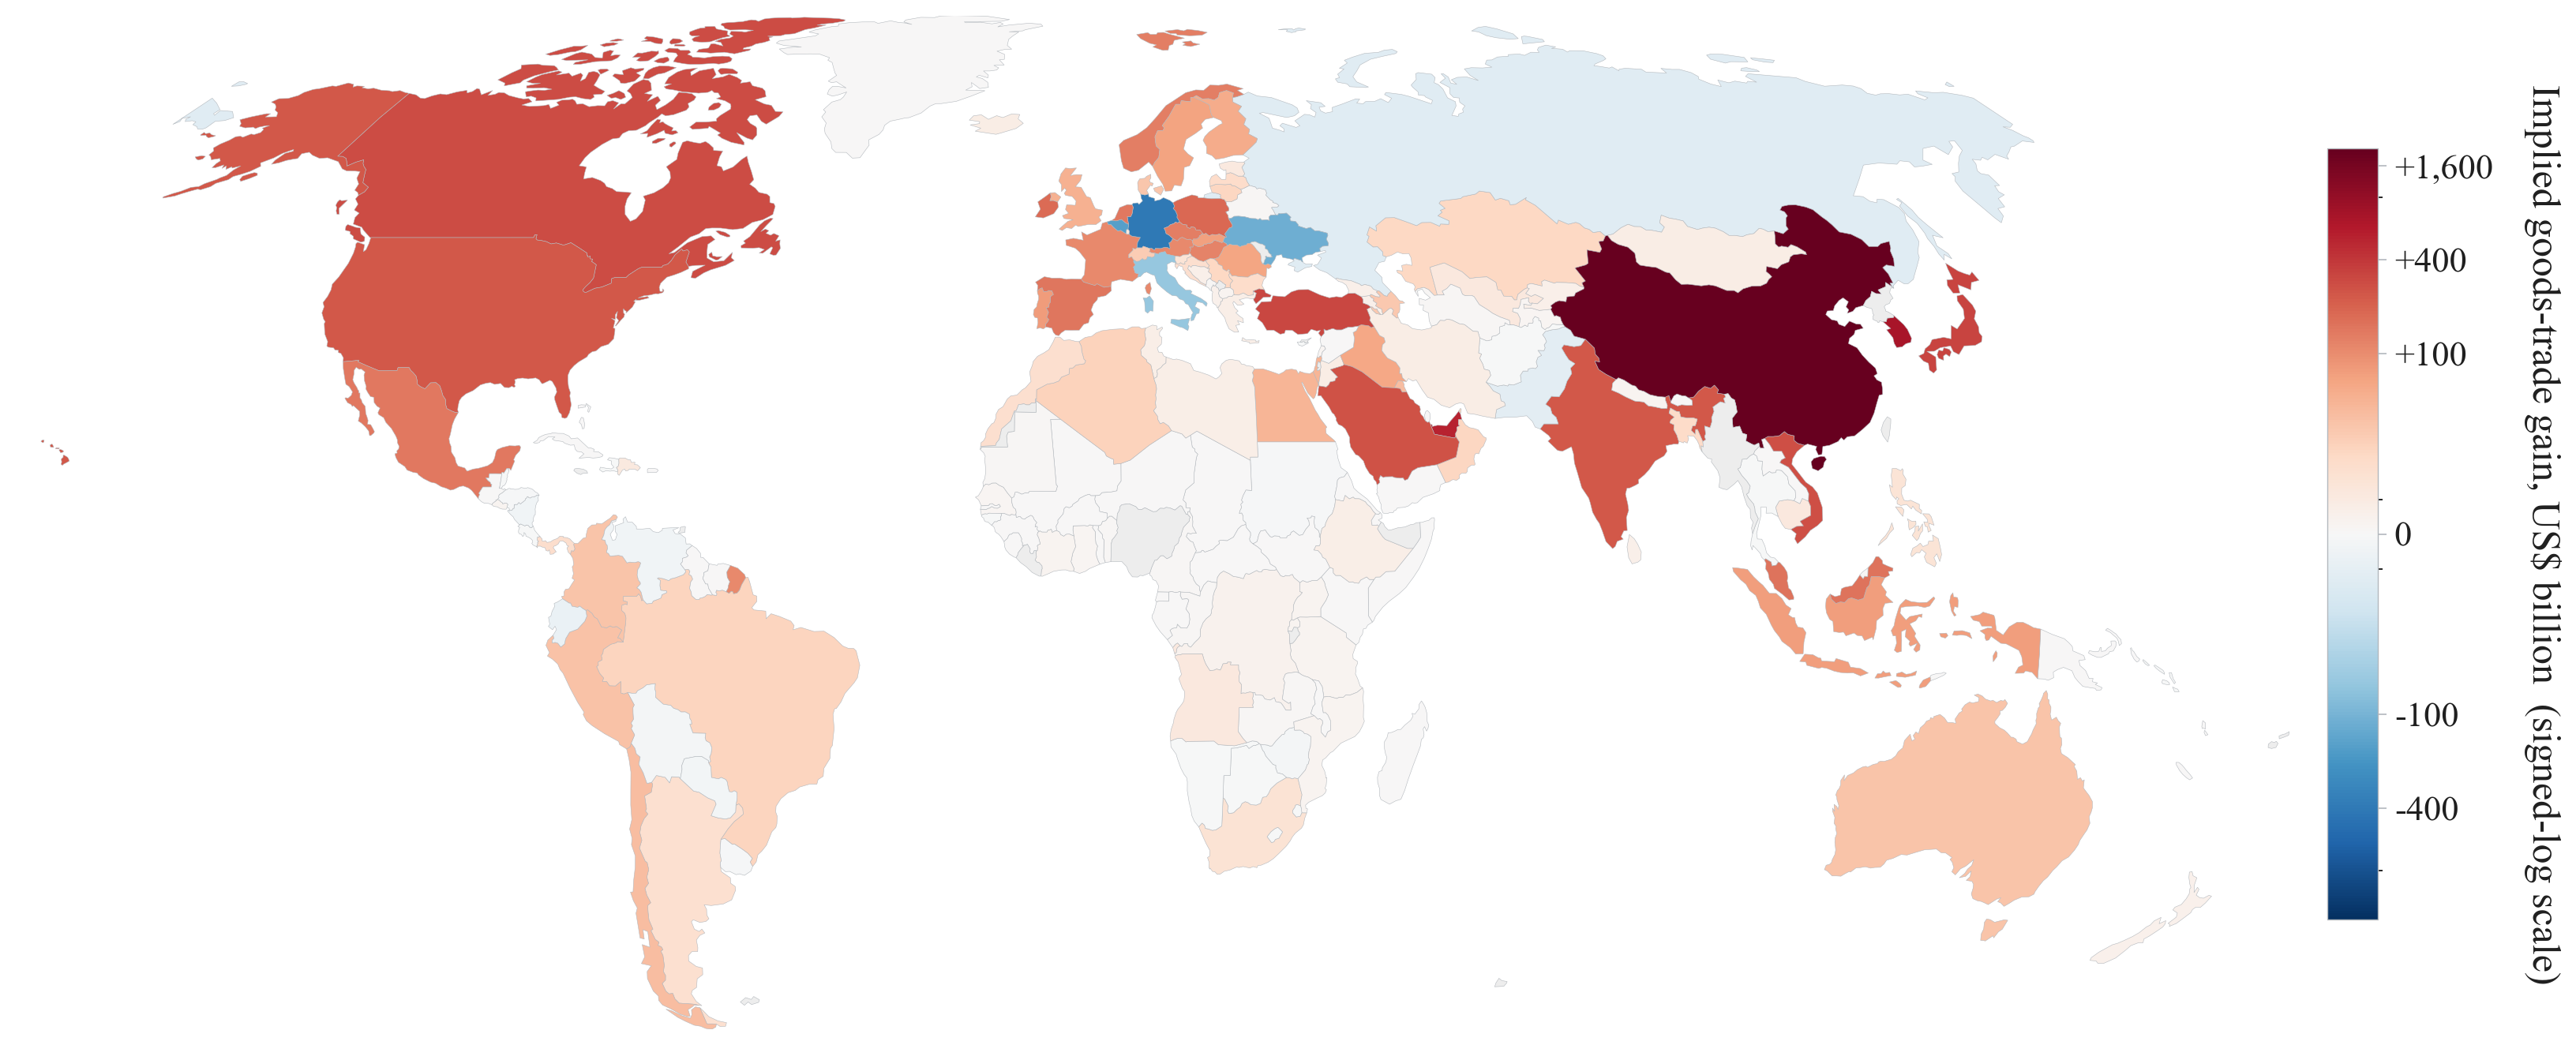
\includegraphics[width=0.92\linewidth]{GACI_implied_map.png}
\caption{GACI-implied goods-trade gain from connectivity growth, 1996--2023,
intensity (openness) channel. Implied gain $=$ goods-trade value
$\times\,(1-\exp(-\beta\,\Delta\ln\text{GACI}_{cwm}))$, $\beta=1.302$.}
\label{fig:impliedmap}
\end{figure}

%=======================================================================
\section{Instrument validity and robustness}
\label{sec:robust}
%=======================================================================
Table~\ref{tab:robust} collects four tests of the identifying assumption.

\paragraph{(A) Over-identification with natural and mixed heritage.} Entering
natural and mixed heritage as two \emph{separate} instruments over-identifies
the single endogenous regressor and licenses a Hansen $J$ test. The two
instruments agree: $J$ is far from rejection for every outcome
($p=0.52$--$0.84$), and the volume elasticity is essentially unchanged
($2.18$, $p<0.01$). The first stage remains adequate (KP $F=8.5$).

\paragraph{(B) Falsification: adding cultural heritage.} Cultural heritage
co-moves with development and historic urban/manufacturing centres, so it is a
plausible exclusion-violator. Adding it as a third instrument moves the Hansen
$J$ to rejection for the volume outcome ($p=0.004$) and toward rejection for
intensity ($p=0.07$), and collapses the point estimate. The data thus
\emph{reject} cultural heritage as a valid instrument---exactly the
discriminating result that supports restricting the instrument to natural and
mixed endowments.

\paragraph{(C) Independent air/sea-distance instrument.} As a fully independent
identification path we construct a Frankel--Romer/Feyrer-type predicted-air-
linkage instrument from geography and the CERDI sea-distance database
\citep{Frankel_1999,Feyrer_2019,Bertoli_2016}. Used alone it delivers a volume
elasticity of $2.26$ ($p<0.01$); combined with the tourism-heritage instrument,
the two completely independent instruments \emph{agree} on the volume channel
($\hat\beta=2.25$, Hansen $J$ $p=0.95$). The intensity channel diverges between
the two instruments ($J$ rejects), which we read as the two instruments
weighting the openness margin differently; we therefore treat the
\emph{volume} elasticity as the most robust quantity and flag the intensity
split transparently.

\paragraph{(D) Temporal stability.} Splitting at the panel midpoint, the
instrument has essentially no first-stage relevance before 2010 (KP
$F=0.3$)---heritage-tourism exposure only began to move hub quality once
low-cost long-haul and Gulf/Asian hub expansion accelerated---while the
post-2010 first stage is strong (KP $F=27.7$). A formal interaction confirms
the connectivity--trade effect is concentrated in the post-2010 period
(interaction on volume $+0.38$, $p<0.01$). We are explicit that identification
is driven by post-2010 variation.

\begin{table}[t]
\centering
\caption{Instrument validity and robustness.}
\label{tab:robust}
\begin{threeparttable}
\small
\begin{tabular}{llccc}
\toprule
 & Instrument set & $\hat\beta$ (volume) & KP $F$ & Hansen $J$ $p$ \\
\midrule
(A) Over-ID, nat+mix      & $z_{\text{nat}},z_{\text{mix}}$ & 2.178\sym{***} & 8.5 & 0.78 \\
(B) Add cultural          & $+\,z_{\text{cult}}$            & 0.394          & 19.8 & 0.004 \\
(C) Air/sea distance only & Feyrer-type                     & 2.257\sym{***} & 153.6 & --- \\
\quad combined            & tourism $+$ Feyrer              & 2.249\sym{***} & 97.2 & 0.95 \\
(D) Pre-2010              & tourism\_int                    & ---            & 0.3 & --- \\
\quad Post-2010           & tourism\_int                    & ---            & 27.7 & --- \\
\bottomrule
\end{tabular}
\begin{tablenotes}\footnotesize
\item All specifications: country and year FE, robust s.e., outcome $=\ln$ goods
volume. (B): cultural heritage is rejected by the over-identification test,
justifying the nat+mix baseline. (C): two independent instruments agree on the
volume channel ($J$ not rejected). (D): first stage is irrelevant pre-2010 and
strong post-2010. \sym{**}~$p<0.05$, \sym{***}~$p<0.01$.
\end{tablenotes}
\end{threeparttable}
\end{table}

%=======================================================================
\section{Heterogeneity: who gains most?}
%=======================================================================
Table~\ref{tab:het} reports interaction-IV estimates in which both
$\ln\text{GACI}_{cwm}$ and its interaction with a mean-centred moderator are
instrumented (by tourism\_int and its interaction, with natural and mixed
entered separately so the Hansen $J$ remains available). Across moderators the
interaction is negative: the connectivity payoff is larger for poorer
(lower baseline GDP per capita), less-connected (lower 1996 hub quality), and
more remote economies. For the intensity channel---where the over-identification
test is satisfied---the income and baseline-connectivity interactions are
negative and significant. We caution that the interacted first stages are
weaker (KP $F\approx2.6$--$4.9$), so the heterogeneity is best read as a
qualitative gradient rather than a precise dose--response.

\begin{table}[t]
\centering
\caption{Heterogeneity: interaction IV, intensity (openness) channel.}
\label{tab:het}
\begin{threeparttable}
\small
\begin{tabular}{lcccc}
\toprule
Moderator (mean-centred) & Connectivity & $\times$ Moderator & KP $F$ & Hansen $J$ $p$ \\
                         & (at mean)    & (interaction)      &        &  \\
\midrule
Baseline income (1996 $\ln$ GDP p.c.)   & 1.576\sym{**} & $-0.265$\sym{**} & 3.6 & 0.45 \\
Baseline connectivity (1996 hub qual.)  & 2.036\sym{*}  & $-1.287$\sym{**} & 2.6 & 0.16 \\
Remoteness ($\ln$ distance to markets)  & 1.586\sym{**} & $-1.508$\sym{**} & 4.9 & 0.51 \\
\bottomrule
\end{tabular}
\begin{tablenotes}\footnotesize
\item Outcome $=\ln(\text{goods}/\text{GDP})$. Both the level and interaction
terms are instrumented; natural and mixed heritage entered separately (over-ID).
Country and year FE; robust s.e. Negative interactions $\Rightarrow$ larger
payoff for poorer, less-connected, more remote countries.
\sym{*}~$p<0.10$, \sym{**}~$p<0.05$.
\end{tablenotes}
\end{threeparttable}
\end{table}

%=======================================================================
\section{Aggregate contribution of two decades of connectivity growth}
%=======================================================================
We translate the intensity elasticity into a partial-equilibrium
counterfactual. For each country the implied gain is
$\text{trade}_{i}\times\bigl(1-\exp(-\beta\,\Delta\ln\text{GACI}^{cwm}_{i})\bigr)$
with $\beta=1.302$, summed across countries. Connectivity growth since 1996 is
associated with about \textbf{\$7.8 trillion} of 2023 goods trade---roughly
\textbf{17\%} of 2023 world goods trade (\$47 trillion) and \textbf{7.4\%} of
2023 world GDP. Equivalently, connectivity growth raised world goods-trade
openness by about 7.4 percentage points of GDP (from roughly 37\% to 45\%).
Figure~\ref{fig:continent} shows the implied intensity gains accrue most to the
Middle East (Gulf hubs) and Asia (China), with the COVID-19 dip visible in
2020--2021. These figures are single-year (2023) attributions of accumulated
1996--2023 connectivity growth, not cumulative flows, and are
partial-equilibrium illustrations that ignore general-equilibrium offsets.

\begin{figure}[t]
\centering
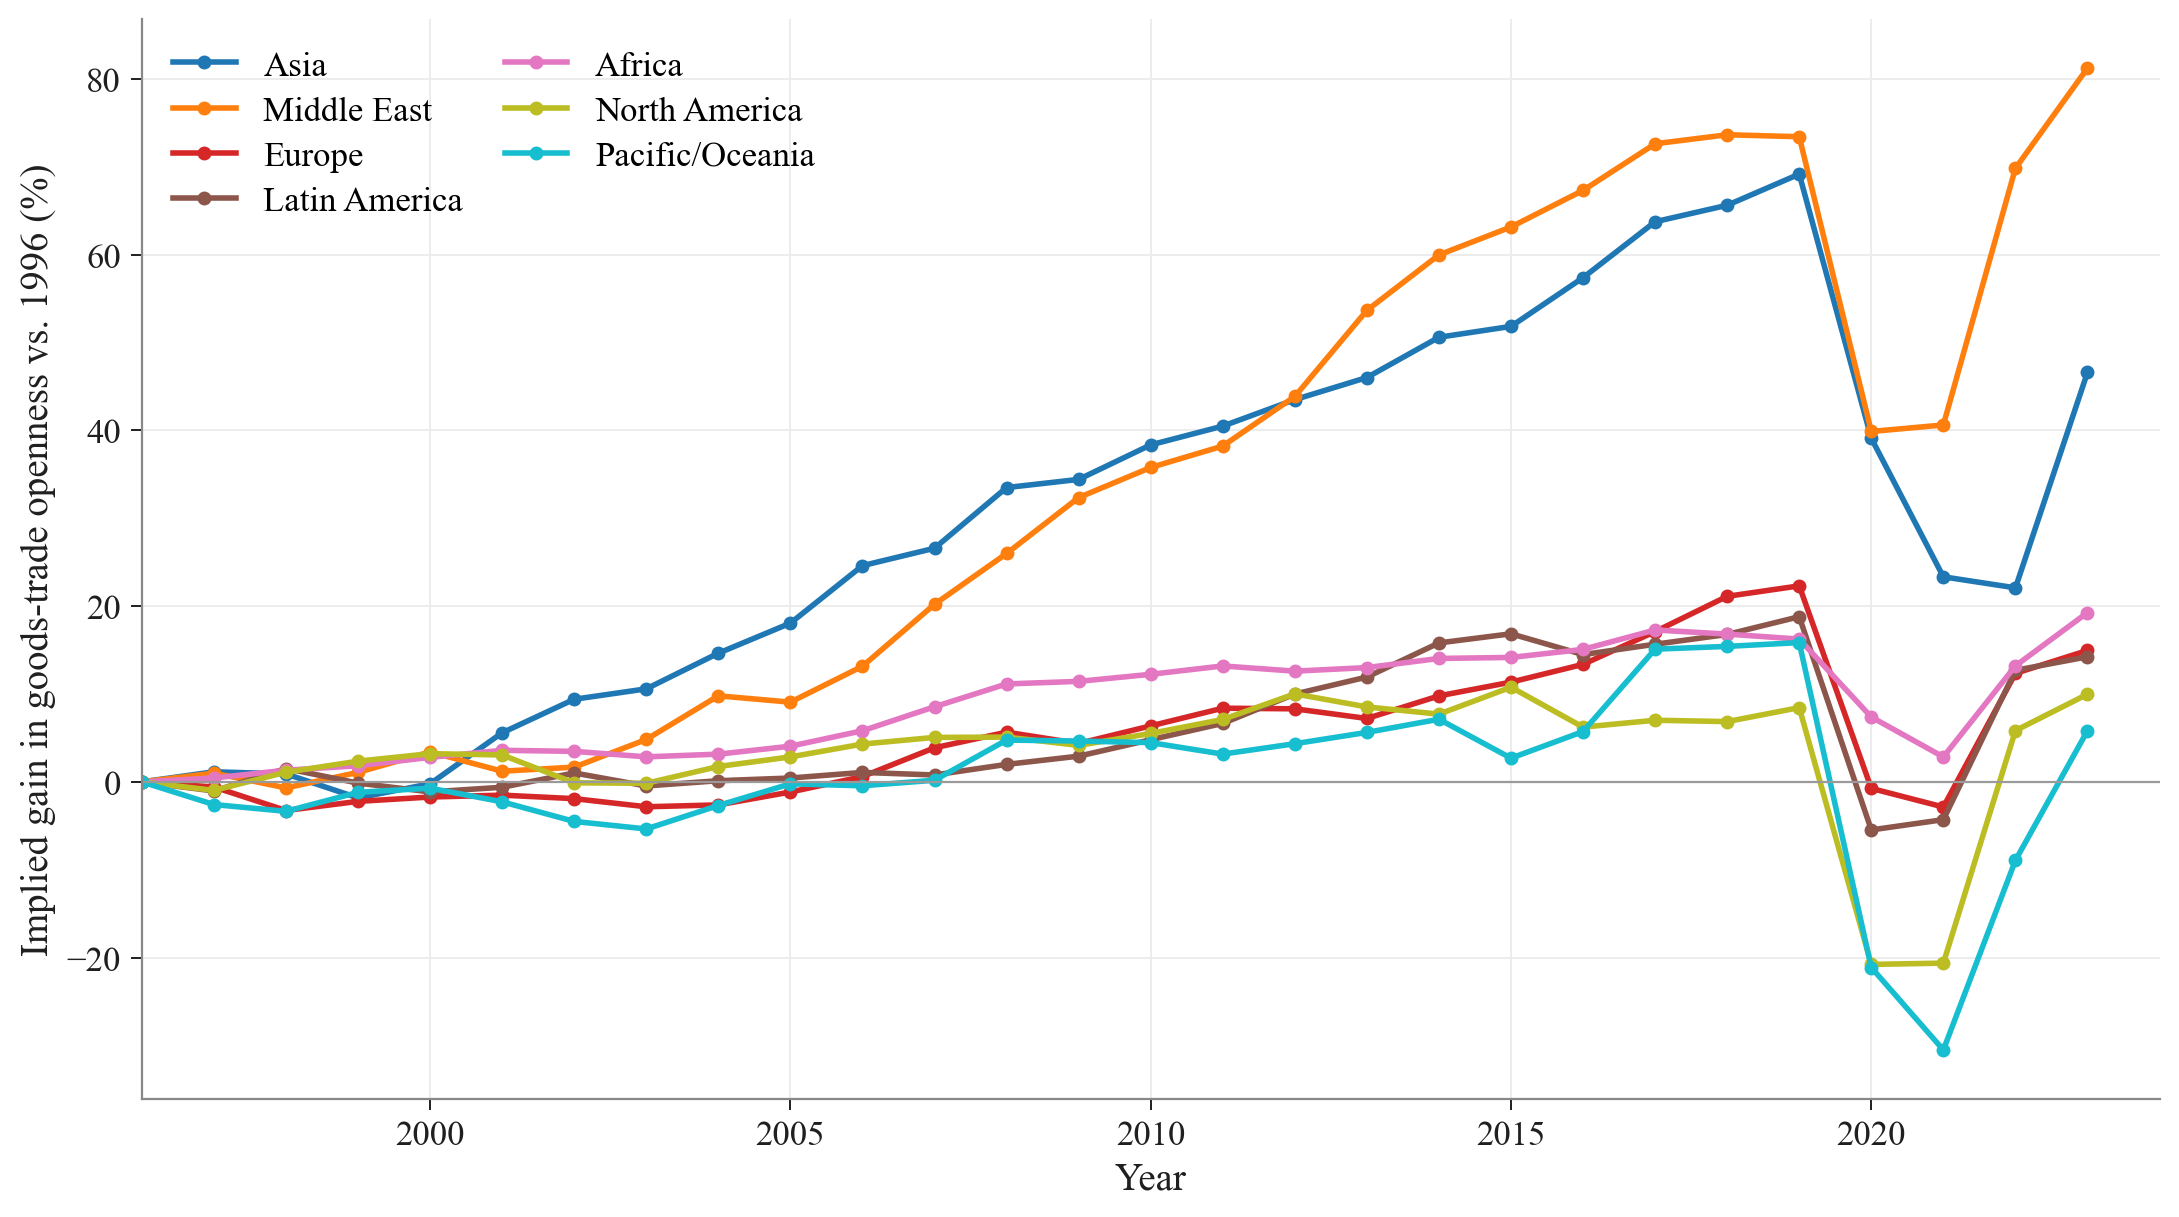
\includegraphics[width=0.92\linewidth]{GACI_continent_trend.png}
\caption{Implied gain in goods-trade openness relative to 1996, by continent,
1996--2023 (intensity channel, $\beta=1.302$; trade-weighted within continent).}
\label{fig:continent}
\end{figure}

%=======================================================================
\section{Connectivity-collapse shocks}
%=======================================================================
For abrupt one-year shocks we measure the connectivity change on
\emph{total} connectivity ($\ln\text{GACI}_{sum}$) with the corresponding sum
intensity elasticity ($0.659$), because hub-quality means are too volatile over
a single year. In the COVID-19 collapse (2019$\to$2020) air connectivity fell
in 140 of 177 countries (median $\Delta\ln\text{GACI}=-0.048$), implying a
goods-trade-flow disruption of about \$1.8 trillion (roughly 4.8\% of 2019
world goods trade), concentrated in major trading hubs
(Figure~\ref{fig:shock}). The Russia--Ukraine episode (2021$\to$2022) was
localised against a globally recovering year, so the net global connectivity
change is positive and not informative as an aggregate loss. These shock
figures are illustrative and we do not rest any structural claim on them.

\begin{figure}[t]
\centering
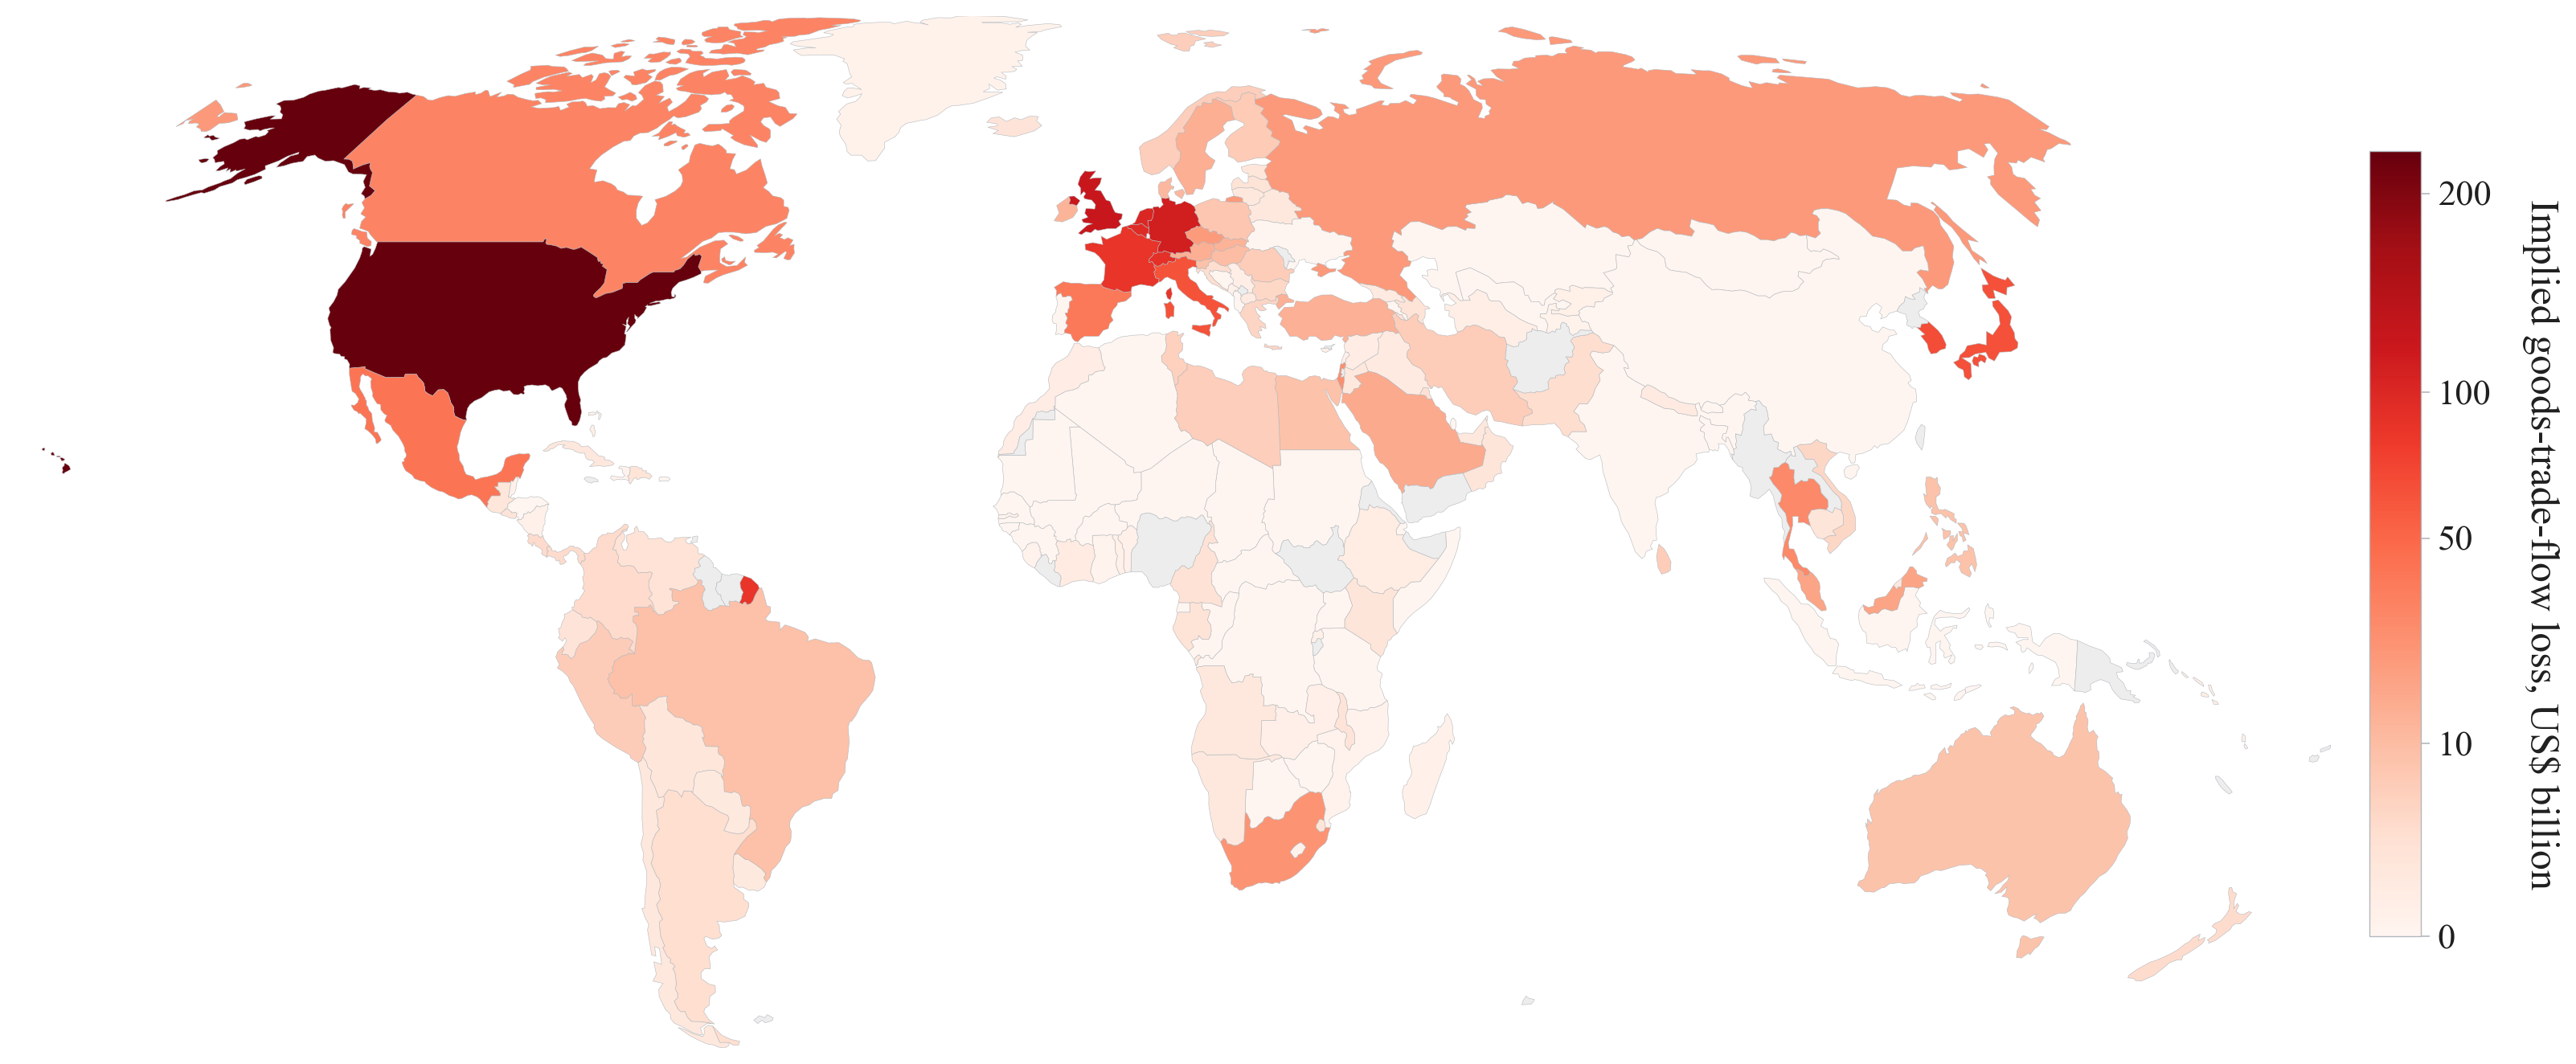
\includegraphics[width=0.92\linewidth]{GACI_shock_map.png}
\caption{COVID-19 (2019$\to$2020): implied goods-trade loss by country from the
air-connectivity collapse. Largest losses fall on major hubs (US, Hong Kong,
Singapore, UK, Germany, Netherlands).}
\label{fig:shock}
\end{figure}

%=======================================================================
\section{Conclusion}
%=======================================================================
Air connectivity is a causal driver of goods-trade integration, not merely a
correlate. Instrumenting a continuous, network-based connectivity index with a
heritage--tourism shift-share instrument, we estimate a goods-volume elasticity
of $2.30$---an intensity (openness) elasticity of $1.30$ plus a GDP-scale
elasticity of $1.00$---that survives over-identification tests, an independent
air/sea-distance instrument, and a cultural-heritage falsification. The payoff
is largest for poorer and under-connected economies, and two decades of
connectivity growth account for on the order of \$7.8 trillion of 2023 goods
trade. The policy implications are direct: airport and route investment and
air-service liberalisation (open-skies agreements) are concrete,
spillover-aware levers for trade and income, with the largest returns in
peripheral economies. Limitations include the partial-equilibrium nature of the
aggregation, the post-2010 concentration of identifying variation, and weaker
first stages in the heterogeneity splits---each a target for future work using
bilateral flows and general-equilibrium gravity structure.

%=======================================================================
\section*{Data and code availability}
%=======================================================================
GACI is derived from proprietary OAG schedule data; the constructed
country-year panel, instrument inputs (UNESCO, WDI, UNWTO, CERDI), and
replication scripts are available from the authors on request.

%=======================================================================
\appendix
\section{Summary statistics}\label{app:sumstat}
%=======================================================================
[Insert \texttt{\_sumstats.csv} as a formatted table: GACI (cwm and sum),
goods-trade openness, GDP per capita, population, heritage counts, tourism
shift; means, s.d., min, max over the 4{,}642 country-year observations.]

\bibliographystyle{elsarticle-harv}
\bibliography{GACI_TRA_refs}

\end{document}
